\documentclass[11pt]{article}

\usepackage[a4paper,margin=1in]{geometry}
\usepackage[T1]{fontenc}
\usepackage[utf8]{inputenc}
\usepackage{lmodern}
\usepackage{microtype}
\usepackage{amsmath,amssymb,amsthm,mathtools}
\usepackage{booktabs}
\usepackage{graphicx}
\usepackage{enumitem}
\usepackage[numbers,sort&compress]{natbib}
\usepackage{xcolor}
\usepackage{xurl}
\usepackage[colorlinks=true,linkcolor=blue!55!black,citecolor=blue!55!black,urlcolor=blue!55!black]{hyperref}
\usepackage[nameinlink,noabbrev]{cleveref}

\setlength{\parindent}{1.4em}
\setlength{\parskip}{0.15em}
\setlist{itemsep=0.25em,topsep=0.35em}

\newtheorem{theorem}{Theorem}[section]
\newtheorem{proposition}[theorem]{Proposition}
\newtheorem{lemma}[theorem]{Lemma}
\newtheorem{corollary}[theorem]{Corollary}
\theoremstyle{definition}
\newtheorem{definition}[theorem]{Definition}
\theoremstyle{remark}
\newtheorem{remark}[theorem]{Remark}

\newcommand{\R}{\mathbb R}
\newcommand{\C}{\mathbb C}
\newcommand{\E}{\mathbb E}
\newcommand{\uc}{u_{\mathrm c}}
\newcommand{\Id}{\operatorname{Id}}
\newcommand{\diag}{\operatorname{diag}}
\newcommand{\spec}{\operatorname{spec}}
\newcommand{\Arg}{\operatorname{Arg}}
\newcommand{\norm}[1]{\left\lVert #1\right\rVert}
\newcommand{\one}{\mathbf 1}

\title{\textbf{Renormalized Spectral Response of Gaussian}\\
\textbf{Quadratic Transfer Matrices}\\
\large Exact Derivatives, Occupation Weighting, and Resolution Scaling}
\author{Liang Wang\\
\small School of Artificial Intelligence and Automation,\\[-0.2em]
\small Huazhong University of Science and Technology, Wuhan 430074, P.R. China\\
\small \texttt{wangliang.f@gmail.com}}
\date{July 2026}

\begin{document}

\maketitle

\begin{abstract}
Logarithmically driven quadratic maps have been studied numerically through
Gaussian-smoothed finite transition matrices.  A preceding analysis proved
that an unweighted fixed-resolution operator average freezes at the limiting
matrix and that its first nonzero renormalized term is a parameter derivative.
The numerical construction, however, accumulates probability flow and then
normalizes each source row.  This produces an occupation-weighted matrix rather
than the unweighted operator average.  We determine exactly when the two have
the same response.

For the row-stochastic Gaussian kernel of the quadratic map
$f_u(x)=1-u x^2$, we derive closed formulas for the first and second parameter
derivatives.  Both derivative matrices have zero row sums.  If a fixed
Gaussian window is retained and renormalized, its exact rowwise
$\ell^1$ error is twice the omitted probability mass.  These identities give
direct finite-difference, normalization, and truncation tests.

For an unanchored schedule
$u_n=\uc+\kappa(\log(n+c))^{-p}+O((\log n)^{-p-1})$, we prove a weighted
slow-variation theorem.  At fixed dimension, every bounded collection of
source weights with positive time density has the same leading response:
\[
  (\log T)^p\bigl(Q_T-K(\uc)\bigr)\longrightarrow \kappa K'(\uc),
\]
row by row, even when the weights are endogenous.  A finite-state
non-autonomous Markov estimator inherits this limit in probability under the
same occupation condition.  Endpoint anchoring is different.  Its leading
term is of order $(\log T)^{-p-1}$ and contains a diagonal matrix of rowwise
logarithmic-age moments; it is generally not the unweighted response.

At fixed physical Gaussian width, midpoint discretization and its first two
parameter derivatives converge at second order, while fixed-window storage
still grows quadratically with grid dimension.  Scaling the width with one
grid cell gives linear storage but changes the limiting operator and destroys
the fixed-norm derivative hypothesis.  Sparse experiments through dimension
$50{,}000$ verify all finite-matrix identities, resolve a stable nonreal
resonance and its eigenphase derivative, and exhibit second-order grid
convergence.  No Riemann-zero ordinates are loaded or compared in these
experiments.  The benchmark width is inherited from a target-informed
exploratory scale and is not an arithmetic prediction; no spectral
realization of the zeros is claimed.
\end{abstract}

\noindent\textbf{Keywords:} quadratic map; transfer matrix; logarithmic
schedule; linear response; non-autonomous Markov chain; sparse eigenvalue
problem; occupation measure.

\medskip
\noindent\textbf{MSC 2020:} 37M25; 37H20; 47A55; 65P20; 60J10.

\section{Introduction}

The prime-dynamics program began with a numerical correspondence between
prime-sieve words and low-dimensional quadratic dynamics
\citep{Wang2026Published}.  Subsequent work separated exact symbolic
statements from admissibility hypotheses, constructed an exact prime kneading
orbit after sparse repair, and isolated the period-two mode at the relevant
band-merging parameter
\citep{WangReformulation2026,WangPrimeSpectrum2026,WangParity2026}.
These results concern sieve words, kneading coordinates, and observable
spectral measures.

A different numerical direction extracts complex eigenvalues from transition
matrices associated with a logarithmically driven quadratic map and compares
their phases with low-lying Riemann-zero ordinates
\citep{WangSpectralFlow2026}.  A theoretical audit established several exact
limitations of such comparisons \citep{WangObstructions2026}.  In particular,
joint pair occupation is not a conditional transition matrix, static sorted
phase unwrapping is an identity, conjugate doubling forces a zero regression
intercept, and a smooth Riemann--von Mangoldt envelope can already produce
excellent relative errors.  That audit also identified a positive object:
for a differentiable finite matrix family $A(u)$,
\[
  (\log T)^p\left(\frac1T\sum_{n\le T}A(u_n)-A(\uc)\right)
  \longrightarrow \kappa A'(\uc).
\]

The remaining gap is structural.  The motivating computation does not average
the matrices $K(u_n)$ uniformly.  It propagates a source distribution,
accumulates the flows $\nu_{n,i}K_{ij}(u_n)$, and only then normalizes each
source row.  The resulting row weights are generated by the same dynamics.
Pointwise continuity of $K$ alone does not identify the limit.

This paper closes that gap at fixed finite resolution for the unanchored
logarithmic schedule.  The mechanism is not mixing but slow variation:
$(\log n)^{-p}$ is asymptotically constant over every positive-density portion
of $\{1,\ldots,T\}$.  Consequently any bounded source weights whose total is
comparable to $T$ preserve the same first derivative.  The theorem applies
pathwise to deterministic expected flows and, after a martingale estimate, in
probability to a finite-state inhomogeneous Markov trajectory.

Endpoint anchoring reveals a complementary effect.  Subtracting the terminal
value cancels the common slowly varying part.  The next coefficient remembers
where in the observation window each source row was occupied.  It is a
logarithmic-age moment and need not be common across rows.  Thus anchoring
improves the nominal decay rate while making occupation bias visible at the
leading surviving order.

\subsection*{Main results}

The contributions are as follows.

\begin{enumerate}[label=\textbf{R\arabic*.},leftmargin=3.2em]
  \item The Gaussian row kernel has exact score formulas for $K'$ and $K''$.
  Both derivative matrices annihilate $\one$, providing stringent
  implementation checks.

  \item Renormalizing a hard Gaussian cutoff changes row $i$ by exactly
  $2q_i$ in $\ell^1$, where $q_i$ is the omitted full-kernel mass.

  \item The row-normalized expected-flow matrix differs from the unweighted
  average by an exact rowwise covariance between source occupation and the
  instantaneous kernel.

  \item For the unanchored logarithmic schedule, every bounded weighting with
  positive density has the same first response.  The result is uniform over
  all such weight arrays and does not require the weights to be independent
  of the dynamics.

  \item A finite-state time-inhomogeneous Markov estimator has sampling error
  $O_{\mathbb P}(T^{-1/2})$, which is smaller than every logarithmic response
  scale.  Positive source occupation therefore suffices to transfer the
  deterministic response to the empirical estimator, and the condition is
  automatic for the full fixed-dimensional Gaussian kernel on a compact
  parameter interval.

  \item For endpoint anchoring, the leading row-$i$ coefficient is
  $p\kappa\beta_i$, where $\beta_i$ is a logarithmic-age moment.  For weights
  proportional to $(n/T)^a$, one has $\beta_i=(a+1)^{-1}$.

  \item Fixed physical noise and cell-scaled noise are different continuum
  paths.  The former gives second-order midpoint consistency but quadratic
  fixed-window storage; the latter gives linear storage while approaching
  deterministic composition in a smooth-observable topology.
\end{enumerate}

\subsection*{Scope}

All derivative and truncation results, together with the weighted response and
finite-state Markov results, are finite-dimensional theorems.  The fixed-width
midpoint statement concerns
a specified smooth integral kernel.  No theorem here identifies that kernel
with a natural self-adjoint operator, and a row-stochastic Gaussian matrix is
not a quantum Hamiltonian.  The numerical section performs no new target fit
and evaluates no zeta zero, but its inherited width is not target-independent.
Nothing here makes a statement about the Riemann hypothesis.

\section{Four finite-time operators and an exact covariance identity}
\label{sec:four}

Let $d\ge2$, let $K_n\in\R^{d\times d}$ be row stochastic, and let
$\nu_n$ be a row probability vector.  In the non-autonomous Markov
interpretation,
\[
  \nu_{n+1}=\nu_n K_n.
\]
There are four natural but generally different finite-time objects:
\begin{align}
  \overline K_T&=\frac1T\sum_{n=1}^T K_n,
  \label{eq:unweighted-average}\\
  C_T&=\frac1T\sum_{n=1}^T\diag(\nu_n)K_n,
  \label{eq:flow-matrix}\\
  Q_T&=D_T^{-1}C_T,\qquad
  D_T=\diag\left(\frac1T\sum_{n=1}^T\nu_n\right),
  \label{eq:weighted-kernel}\\
  \Pi_T&=K_1K_2\cdots K_T.
  \label{eq:product}
\end{align}
The last convention acts on row distributions.  The matrix $C_T$ is expected
joint flow, $Q_T$ is its row-conditional normalization, and $\Pi_T$ retains
operator order.  Their spectra need not agree.

Write $K_{n,i\bullet}$ for row $i$, and define
\[
  \overline\nu_{i,T}=\frac1T\sum_{n=1}^T\nu_{n,i}.
\]

\begin{proposition}[Exact occupation covariance]\label{prop:covariance}
If $\overline\nu_{i,T}>0$, then
\begin{equation}\label{eq:covariance}
  Q_{T,i\bullet}-\overline K_{T,i\bullet}
  =
  \frac{
    T^{-1}\sum_{n=1}^T
    (\nu_{n,i}-\overline\nu_{i,T})
    (K_{n,i\bullet}-\overline K_{T,i\bullet})
  }{\overline\nu_{i,T}}.
\end{equation}
Thus occupation weighting is absent exactly when the displayed rowwise
covariance vanishes.
\end{proposition}

\begin{proof}
Expand the numerator in \eqref{eq:covariance}.  It equals
\[
  \frac1T\sum_n\nu_{n,i}K_{n,i\bullet}
  -\overline\nu_{i,T}\overline K_{T,i\bullet}.
\]
Division by $\overline\nu_{i,T}$ gives \eqref{eq:weighted-kernel} minus
\eqref{eq:unweighted-average}.
\end{proof}

\begin{remark}[Sparse row normalization]\label{rem:csr}
For a compressed sparse row matrix, the array of stored indices contains
\emph{column} indices.  Correct normalization multiplies the stored values by
the row factors repeated according to consecutive differences of the row
pointer.  Indexing row sums by the column-index array instead performs a
destination-dependent rescaling and does not produce a stochastic matrix.
The reproducibility implementation tests this distinction explicitly.  The
numerical values reported below are newly computed with row-pointer
normalization and are not a reproduction of earlier phase-fit lists.
\end{remark}

\section{The Gaussian quadratic family}
\label{sec:gaussian}

Let
\[
  I=[-1,1],\qquad
  c_i=-1+\left(i-\frac12\right)h,\qquad
  h=\frac2d,\qquad 1\le i\le d.
\]
For $f_u(x)=1-u x^2$ and fixed $\sigma>0$, put
\begin{align}
  m_i(u)&=f_u(c_i)=1-u c_i^2,\label{eq:mean}\\
  w_{ij}(u)&=\exp\left(
    -\frac{(c_j-m_i(u))^2}{2\sigma^2}
  \right),\label{eq:weight}\\
  K_{ij}(u)&=\frac{w_{ij}(u)}{Z_i(u)},\qquad
  Z_i(u)=\sum_{k=1}^d w_{ik}(u).
  \label{eq:kernel}
\end{align}
Every entry is positive and analytic in $u$, and $K(u)\one=\one$.

\subsection{Exact first and second derivatives}

Define
\begin{equation}\label{eq:score}
  a_{ij}(u)=\partial_u\log w_{ij}(u)
  =-\frac{c_i^2}{\sigma^2}\bigl(c_j-m_i(u)\bigr),
  \qquad
  \overline a_i(u)=\sum_kK_{ik}(u)a_{ik}(u).
\end{equation}

\begin{theorem}[Gaussian score identities]\label{thm:derivatives}
The first two derivatives of \eqref{eq:kernel} are
\begin{align}
  K'_{ij}(u)
  &=K_{ij}(u)\bigl(a_{ij}(u)-\overline a_i(u)\bigr),
  \label{eq:first-derivative}\\
  K''_{ij}(u)
  &=K_{ij}(u)\left[
    \bigl(a_{ij}(u)-\overline a_i(u)\bigr)^2
    -\operatorname{Var}_{K_i(u)}(a_i(u))
  \right].
  \label{eq:second-derivative}
\end{align}
In particular,
\begin{equation}\label{eq:zero-row-sums}
  K'(u)\one=0,\qquad K''(u)\one=0.
\end{equation}
\end{theorem}

\begin{proof}
Logarithmic differentiation of $K_{ij}=w_{ij}/Z_i$ gives
\[
  \partial_u\log K_{ij}=a_{ij}-\overline a_i,
\]
which proves \eqref{eq:first-derivative}.  Moreover,
\[
  \partial_u a_{ij}=-\frac{c_i^4}{\sigma^2}
\]
is constant in $j$ for fixed row $i$.  Differentiating
\eqref{eq:first-derivative}, the centered contribution from
$\partial_u a_{ij}$ therefore cancels.  The derivative of
$\overline a_i$ contributes
$\operatorname{Var}_{K_i}(a_i)$, proving
\eqref{eq:second-derivative}.  Summing the two formulas over $j$ proves
\eqref{eq:zero-row-sums}.
\end{proof}

The formulas also identify the response scale without a finite difference.
Let $Z_i$ be the row-$i$ random variable taking value
$c_j-m_i(u)$ with probability $K_{ij}(u)$.

\begin{proposition}[Exact derivative norms]\label{prop:derivative-norms}
For every row,
\begin{align}
  \sum_j|K'_{ij}(u)|
  &=
  \frac{c_i^2}{\sigma^2}
  \E\left|Z_i-\E Z_i\right|,
  \label{eq:first-norm}\\
  \sum_j|K''_{ij}(u)|
  &=
  \frac{c_i^4}{\sigma^4}
  \E\left|
    (Z_i-\E Z_i)^2-\operatorname{Var}(Z_i)
  \right|.
  \label{eq:second-norm}
\end{align}
\end{proposition}

\begin{proof}
By \eqref{eq:score},
$a_{ij}-\overline a_i=-c_i^2(Z_i-\E Z_i)/\sigma^2$.
Substitution into \eqref{eq:first-derivative} and
\eqref{eq:second-derivative} gives the two identities.
\end{proof}

\begin{remark}[The norm matters when the noise shrinks]\label{rem:norm}
For an interior row resolved by several cells, the typical centered
displacement is of order $\sigma$.  Equations
\eqref{eq:first-norm}--\eqref{eq:second-norm} then give the characteristic
scales $\norm{K'}_\infty=O(\sigma^{-1})$ and
$\norm{K''}_\infty=O(\sigma^{-2})$.  Thus a family with
$\sigma=\sigma_d\to0$ need not have a uniformly bounded derivative in raw
matrix $\ell^\infty$ norm, even though its action on smooth observables may
converge.  A resolution-time response theorem must specify the common
operator topology.
\end{remark}

\subsection{Exact cutoff error}

Let $S_i\subset\{1,\ldots,d\}$ be a nonempty retained set for row $i$, and
renormalize the full kernel on that set:
\begin{equation}\label{eq:truncated-kernel}
  K^S_{ij}=
  \begin{cases}
    K_{ij}/(1-q_i),&j\in S_i,\\
    0,&j\notin S_i,
  \end{cases}
  \qquad
  q_i=\sum_{j\notin S_i}K_{ij}.
\end{equation}

\begin{proposition}[Twice-the-tail identity]\label{prop:tail}
For every row,
\begin{equation}\label{eq:tail-identity}
  \sum_j|K_{ij}-K^S_{ij}|=2q_i.
\end{equation}
Consequently
\begin{equation}\label{eq:tail-infinity}
  \norm{K-K^S}_\infty=2\max_iq_i.
\end{equation}
\end{proposition}

\begin{proof}
On the retained set, $K^S_{ij}-K_{ij}=K_{ij}q_i/(1-q_i)$,
whose sum is $q_i$.  The omitted entries also sum to $q_i$.
\end{proof}

\begin{remark}[Nonnormal spectral caution]\label{rem:nonnormal}
The norm estimate \eqref{eq:tail-infinity} is an operator statement, not an
unconditional one-to-one eigenvalue bound.  Gaussian Markov matrices are
generally nonnormal.  A simple eigenvalue has a first-order condition number
determined by its left-right overlap, while a global eigenvalue enclosure
requires a resolvent or a diagonalizability estimate
\citep{Kato1995,StewartSun1990}.
\end{remark}

\subsection{Simple resonance and eigenphase response}

Let $\lambda(u)\ne0$ be a simple eigenvalue near $u=\uc$, with
\[
  K(\uc)r=\lambda r,\qquad
  \ell^*K(\uc)=\lambda\ell^*,\qquad
  \ell^*r=1.
\]
Analytic matrix perturbation theory gives
\begin{equation}\label{eq:eigen-derivative}
  \lambda'(\uc)=\ell^*K'(\uc)r,
  \qquad
  \theta'(\uc)=
  \operatorname{Im}\frac{\ell^*K'(\uc)r}{\lambda},
  \quad \theta=\Arg\lambda.
\end{equation}
These are responses of a finite Markov resonance.  They do not turn its phase
into an energy.

\section{Weighted logarithmic response}
\label{sec:weighted}

Put
\[
  L_T=\log(T+c),\qquad s_T=L_T^{-p},
\]
where $c>1$ and $p>0$.  The following uniform weighted form of slow
variation is the key step.  It is a concrete Cesaro property of a slowly
varying sequence \citep{BinghamGoldieTeugels1987}.

\begin{lemma}[Positive-density weighted slow variation]
\label{lem:weighted-slow}
Let $0\le a_{n,T}\le M$ and
$A_T=\sum_{n=1}^T a_{n,T}\ge\alpha T$ for fixed $M,\alpha>0$.
Then, uniformly over all such triangular weight arrays,
\begin{equation}\label{eq:weighted-slow}
  \frac1{A_T}\sum_{n=1}^Ta_{n,T}
  \frac{L_T^p}{(\log(n+c))^p}
  \longrightarrow1.
\end{equation}
The same assertion holds with $p$ replaced by every positive exponent.
\end{lemma}

\begin{proof}
The ratio in \eqref{eq:weighted-slow} is at least one.  Therefore its
weighted mean excess is bounded by
\[
  \frac{M}{\alpha}
  \left[
    \frac1T\sum_{n=1}^T
    \frac{L_T^p}{(\log(n+c))^p}-1
  \right].
\]
The bracket tends to zero by the logarithmic Cesaro asymptotic
\[
  \frac1T\sum_{n=1}^T(\log(n+c))^{-p}
  =L_T^{-p}\bigl(1+O(L_T^{-1})\bigr).
\]
\end{proof}

Consider
\begin{equation}\label{eq:unanchored-schedule}
  u_n=\uc+\delta_n,\qquad
  \delta_n=
  \frac{\kappa}{(\log(n+c))^p}
  +O\left((\log(n+c))^{-p-1}\right).
\end{equation}
The error is assumed uniform in $n$ once a fixed initial segment is removed.
For each source row $i$, allow arbitrary weights $a_{n,i,T}\in[0,M]$ and set
\begin{equation}\label{eq:general-weighted-row}
  Q_{T,i\bullet}
  =
  \frac{\sum_{n=1}^T a_{n,i,T}K_{i\bullet}(u_n)}
       {\sum_{n=1}^T a_{n,i,T}}.
\end{equation}

\begin{theorem}[Occupation-universal unanchored response]
\label{thm:unanchored}
Assume $K(u)$ is differentiable at $\uc$ and bounded along the schedule.
For fixed $d$, suppose that for every row
\begin{equation}\label{eq:positive-density}
  \sum_{n=1}^T a_{n,i,T}\ge\alpha_iT
\end{equation}
for all sufficiently large $T$, with $\alpha_i>0$.  Then
\begin{equation}\label{eq:unanchored-response}
  L_T^p\bigl(Q_T-K(\uc)\bigr)
  \longrightarrow \kappa K'(\uc)
\end{equation}
in matrix infinity norm.  The conclusion is uniform over all weights
satisfying the displayed bounds.
\end{theorem}

\begin{proof}
Differentiability gives, row by row,
\[
  K_{i\bullet}(\uc+t)
  =K_{i\bullet}(\uc)+tK'_{i\bullet}(\uc)+r_i(t),
  \qquad
  \frac{\norm{r_i(t)}_1}{|t|}\longrightarrow0.
\]
By \cref{lem:weighted-slow}, the weighted mean of $\delta_n/s_T$
converges to $\kappa$.  Applying the same lemma with exponent $p+1$
shows that the error term in \eqref{eq:unanchored-schedule} contributes
$O(L_T^{-1})$ after division by $s_T$.

For the Taylor remainder, fix $\varepsilon>0$ and choose $N$ so that
$\norm{r_i(\delta_n)}_1\le\varepsilon|\delta_n|$ for $n\ge N$.
The first $N-1$ terms contribute
$O((Ts_T)^{-1})=o(1)$ after weighted normalization, while the remaining
terms are bounded by $\varepsilon$ times a uniformly bounded weighted mean
of $|\delta_n|/s_T$.  Letting $\varepsilon\downarrow0$ proves the row
limit.  Since $d$ is fixed, the maximum over rows gives
\eqref{eq:unanchored-response}.
\end{proof}

\begin{corollary}[Expected-flow normalization]\label{cor:expected-flow}
Let $\nu_n$ be any sequence of source probability vectors and put
$a_{n,i,T}=\nu_{n,i}$.  If
\[
  \liminf_{T\to\infty}\frac1T\sum_{n=1}^T\nu_{n,i}>0
\]
for every fixed row, then the row-normalized expected-flow matrix
\eqref{eq:weighted-kernel} satisfies \eqref{eq:unanchored-response}.
No independence, stationarity, or mixing of the weights is required.
\end{corollary}

This corollary applies directly to a propagated probability cloud.  A
single random trajectory adds transition noise, handled next.

\begin{corollary}[One inhomogeneous Markov trajectory]
\label{cor:markov}
Let $(X_n)$ be a finite-state time-inhomogeneous Markov chain with
\[
  \mathbb P(X_{n+1}=j\mid X_1,\ldots,X_n)
  =K_{X_nj}(u_n).
\]
Define source counts and the empirical conditional matrix by
\begin{align}
  N_{i,T}&=\sum_{n=1}^T\mathbf1_{\{X_n=i\}},\\
  \widehat K_{ij,T}
  &=\frac{\sum_{n=1}^T
    \mathbf1_{\{X_n=i,X_{n+1}=j\}}}{N_{i,T}}.
\end{align}
Suppose that for every $i$ there is $\alpha_i>0$ such that
\begin{equation}\label{eq:random-occupation}
  \mathbb P(N_{i,T}\ge\alpha_iT)\longrightarrow1.
\end{equation}
Then
\begin{equation}\label{eq:markov-response}
  L_T^p\bigl(\widehat K_T-K(\uc)\bigr)
  \longrightarrow\kappa K'(\uc)
\end{equation}
in probability.
\end{corollary}

\begin{proof}
Condition on the realized source indicators and define
\[
  M_{ij,T}=\sum_{n=1}^T\mathbf1_{\{X_n=i\}}
  \left(\mathbf1_{\{X_{n+1}=j\}}-K_{ij}(u_n)\right).
\]
This is a martingale with bounded increments and
$\E|M_{ij,T}|^2\le T$.  On the event in \eqref{eq:random-occupation},
\[
  \frac{M_{ij,T}}{N_{i,T}}=O_{\mathbb P}(T^{-1/2})
  =o_{\mathbb P}(L_T^{-p}).
\]
The conditional mean term is \eqref{eq:general-weighted-row} with
$a_{n,i,T}=\mathbf1_{\{X_n=i\}}$, so \cref{thm:unanchored} applies on
the same event.  There are finitely many entries.
\end{proof}

\begin{corollary}[Full Gaussian positivity supplies occupation]
\label{cor:gaussian-occupation}
Fix $d<\infty$ and $\sigma>0$, and let the parameters $u_n$ remain in a
compact interval $J$.  For the full kernel \eqref{eq:kernel}, the occupation
conditions in \cref{cor:expected-flow,cor:markov} hold automatically.
Consequently both conclusions apply without a separate occupation
hypothesis.
\end{corollary}

\begin{proof}
Continuity, strict positivity, and finiteness give
\[
  \varepsilon=\min_{u\in J}\min_{i,j}K_{ij}(u)>0.
\]
For a propagated source distribution,
$\nu_{n+1,i}=\sum_j\nu_{n,j}K_{ji}(u_n)\ge\varepsilon$.
For a Markov trajectory, put
$p_{n,i}=\mathbb P(X_n=i\mid X_1,\ldots,X_{n-1})\ge\varepsilon$.
The sum
\[
  \sum_{n=2}^T\bigl(\mathbf1_{\{X_n=i\}}-p_{n,i}\bigr)
\]
is a bounded-increment martingale and is $o_{\mathbb P}(T)$.
Thus $N_{i,T}/T\ge\varepsilon+o_{\mathbb P}(1)$.
\end{proof}

\begin{remark}[What the occupation condition does not give]
\label{rem:occupation-limit}
At fixed $d$, strict Gaussian positivity makes positive occupation plausible,
and \cref{cor:gaussian-occupation} makes it automatic for the full kernel.
A hard sparse cutoff introduces exact zeros, so its occupation condition must
again be checked.  In either case, the lower bound is not uniform for free
when $d\to\infty$: source probabilities must sum to one, so a common lower
density cannot remain independent of $d$.  The theorem therefore closes the
fixed-resolution occupation gap but does not interchange the long-time and
continuum limits.
\end{remark}

\section{Endpoint anchoring exposes logarithmic age}
\label{sec:anchored}

For a triangular schedule ending exactly at $\uc$, define
\begin{equation}\label{eq:anchored-schedule}
  u_{n,T}=\uc+\delta_{n,T},\qquad
  \delta_{n,T}=\kappa\left[
    \frac1{(\log(n+c))^p}-\frac1{L_T^p}
  \right].
\end{equation}
The unweighted average has coefficient $p\kappa L_T^{-p-1}$.
Weighted rows need not have the same coefficient.

For row weights $a_{n,i,T}$, let
\begin{equation}\label{eq:log-age}
  r_{n,T}=\log\frac{T+c}{n+c},\qquad
  \beta_{i,T}=
  \frac{\sum_{n=1}^Ta_{n,i,T}r_{n,T}}
       {\sum_{n=1}^Ta_{n,i,T}}.
\end{equation}

\begin{theorem}[Anchored occupation response]\label{thm:anchored}
Assume the boundedness and positive-density conditions of
\cref{thm:unanchored}.  Suppose in addition that, for every row,
\begin{equation}\label{eq:age-assumptions}
  \beta_{i,T}\longrightarrow\beta_i,\qquad
  \frac{\sum_{n=1}^Ta_{n,i,T}r_{n,T}^2}
       {\sum_{n=1}^Ta_{n,i,T}}=O(1).
\end{equation}
If $K$ is differentiable at $\uc$, then
\begin{equation}\label{eq:anchored-matrix-response}
  L_T^{p+1}\bigl(Q_T-K(\uc)\bigr)
  \longrightarrow p\kappa B K'(\uc),
  \qquad
  B=\diag(\beta_1,\ldots,\beta_d).
\end{equation}
\end{theorem}

\begin{proof}
Since $\log(n+c)=L_T-r_{n,T}$, Taylor expansion gives
\[
  (\log(n+c))^{-p}-L_T^{-p}
  =p\,r_{n,T}L_T^{-p-1}
   +O(r_{n,T}^2L_T^{-p-2})
\]
whenever $n\ge T^{1/2}$.  The total weighted contribution of
$n<T^{1/2}$ is $o(L_T^{-p-1})$ because the weights are bounded and
their denominator is at least $\alpha_iT$.  Averaging the expansion and
using \eqref{eq:age-assumptions} yields
\[
  \frac{\sum_na_{n,i,T}\delta_{n,T}}{\sum_na_{n,i,T}}
  =
  \frac{p\kappa\beta_i+o(1)}{L_T^{p+1}}.
\]
The differentiability remainder is handled as in
\cref{thm:unanchored}; the weighted mean absolute displacement has the
same $O(L_T^{-p-1})$ scale under \eqref{eq:age-assumptions}.
This proves each row of \eqref{eq:anchored-matrix-response}.
\end{proof}

\begin{corollary}[Power-profile weights]\label{cor:power}
If $a_{n,i,T}=(n/T)^{a_i}$ with $a_i\ge0$, then
\begin{equation}\label{eq:power-age}
  \beta_i=
  \frac{\int_0^1x^{a_i}(-\log x)\,dx}
       {\int_0^1x^{a_i}\,dx}
  =\frac1{a_i+1}.
\end{equation}
The unweighted row has $\beta_i=1$, while a row occupied later in the
window has $\beta_i<1$.
\end{corollary}

\begin{proof}
Both weighted sums in \eqref{eq:log-age}, after division by $T$, are
improper Riemann sums with integrable logarithmic moments.  The displayed
integrals equal $(a_i+1)^{-2}$ and $(a_i+1)^{-1}$, respectively.
\end{proof}

\begin{corollary}[Anchored resonance response]\label{cor:anchored-eigen}
Let $\lambda\ne0$ be a simple eigenvalue of $K(\uc)$ with normalized left
and right eigenvectors $\ell,r$.  Under \cref{thm:anchored}, the
corresponding eigenvalue $\lambda_T$ of $Q_T$ satisfies
\begin{align}
  L_T^{p+1}(\lambda_T-\lambda)
  &\longrightarrow p\kappa\,\ell^*BK'(\uc)r,\label{eq:anchored-eigen}\\
  L_T^{p+1}(\Arg\lambda_T-\Arg\lambda)
  &\longrightarrow
  p\kappa\,\operatorname{Im}
  \frac{\ell^*BK'(\uc)r}{\lambda}.
  \label{eq:anchored-phase}
\end{align}
Only when $B$ is scalar on the relevant rows does this reduce to the
unweighted anchored coefficient.
\end{corollary}

\section{Resolution scaling and the sparsity tradeoff}
\label{sec:resolution}

\subsection{Fixed physical width}

For fixed $\sigma>0$, define the continuum Markov operator on
$I=[-1,1]$ by
\begin{equation}\label{eq:continuum-kernel}
  (\mathcal K_{\sigma,u}g)(x)=
  \frac{\int_{-1}^1
    e^{-(y-f_u(x))^2/(2\sigma^2)}g(y)\,dy}
       {\int_{-1}^1
    e^{-(y-f_u(x))^2/(2\sigma^2)}\,dy}.
\end{equation}
The full matrix \eqref{eq:kernel} is its midpoint quotient quadrature.

\begin{proposition}[Second-order midpoint consistency]
\label{prop:midpoint}
Let $u$ range over a compact interval and keep $\sigma>0$ fixed.
For every $g\in C^2(I)$,
\begin{equation}\label{eq:midpoint}
  \max_i\left|
    \sum_jK_{ij}^{(d,\sigma)}(u)g(c_j)
    -(\mathcal K_{\sigma,u}g)(c_i)
  \right|
  \le C_{\sigma,u}\,h^2\norm{g}_{C^2}.
\end{equation}
The same conclusion holds after one or two parameter derivatives, with
constants depending on $\sigma$ and the compact parameter interval.
\end{proposition}

\begin{proof}
Multiply numerator and denominator of \eqref{eq:kernel} by $h$.
Composite midpoint quadrature has error $O(h^2)$ for the smooth numerator
and denominator integrands.  The continuum denominator is uniformly
positive for $x\in I$ and $u$ in a compact interval.  The quotient estimate
follows.  Parameter differentiation only multiplies the Gaussian by smooth
polynomials in $x,y$, so the same argument applies twice.
\end{proof}

This proposition concerns the full Gaussian sum.  A fixed $L\sigma$ cutoff
adds the explicit error from \cref{prop:tail}.  To converge to the exact
full kernel in operator norm as $d\to\infty$, the omitted mass must also be
sent to zero; choosing $L=6$ makes it numerically small but not
mathematically zero.

\subsection{Fixed width is not asymptotically sparse}

Suppose a support fixed at $u=\uc$ retains every center in
\[
  |c_j-m_i(\uc)|\le L\sigma+\Delta c_i^2,
\]
where $\Delta$ covers a parameter neighborhood.  An interval of radius $R$
contains at most $1+2R/h$ midpoint centers.

\begin{proposition}[Storage dichotomy]\label{prop:storage}
Assume $\uc\in(0,2)$.
The number of retained entries satisfies
\begin{equation}\label{eq:nnz-bound}
  \operatorname{nnz}(K)
  \le d\left(1+\frac{2(L\sigma+\Delta)}h\right).
\end{equation}
For fixed positive $\sigma$ and fixed $L$, a positive fraction of interior
rows has $\Theta(d)$ retained entries, so
$\operatorname{nnz}(K)=\Theta(d^2)$.  If instead
$\sigma_d=qh$ and $\Delta_d=O(h)$, then
$\operatorname{nnz}(K)=O(d)$.
\end{proposition}

\begin{proof}
The upper bound follows from counting grid centers in each retained
interval and using $c_i^2\le1$.  For fixed $\sigma$, rows whose means stay a
fixed distance from the boundary retain an interval of fixed positive
length, hence $\Theta(d)$ centers.  If $\sigma_d$ and $\Delta_d$ are
$O(h)$, the parenthesis in \eqref{eq:nnz-bound} is bounded independently of
$d$.
\end{proof}

\begin{remark}[The two paths have different limits]\label{rem:two-paths}
At fixed $\sigma$, \cref{prop:midpoint} approaches the noisy integral
operator \eqref{eq:continuum-kernel}.  If $\sigma_d=qh\to0$, then for every
continuous $g$ and every row whose image remains in $I$, the Gaussian
average concentrates and approaches $g(f_u(c_i))$.  The limit is
deterministic composition on smooth observables.  Meanwhile
\cref{prop:derivative-norms} shows why raw matrix derivative norms can grow.
Linear storage is therefore obtained by changing both the limiting operator
and the topology in which response can remain bounded.  It is not a cheaper
discretization of the same fixed-noise limit.
\end{remark}

\section{Reproducible sparse experiments}
\label{sec:experiments}

\subsection{Protocol}

The implementation uses the exact formulas
\eqref{eq:first-derivative}--\eqref{eq:second-derivative} on a support pattern
fixed at $\uc$.  Fixing the pattern prevents artificial finite-difference
jumps when an entry crosses the cutoff.  All matrices are compressed sparse
row arrays.  The tests verify:
\begin{enumerate}[label=(\roman*),leftmargin=2.2em]
  \item row sums of $K$, $K'$, and $K''$ are $1$, $0$, and $0$;
  \item analytic derivatives agree with centered finite differences;
  \item sparse full-support output agrees with an independent dense
  reference;
  \item cutoff error obeys \eqref{eq:tail-identity};
  \item row-pointer normalization differs from column-index rescaling; and
  \item weighted schedule coefficients approach the limits in
  \cref{thm:unanchored,thm:anchored}.
\end{enumerate}
All ten tests pass.

The benchmark parameters are
\[
  \uc=1.5437,\qquad \sigma=0.00785,\qquad L=6.
\]
The width is retained from the exploratory numerical scale only as a
fixed-noise benchmark.  That historical scale was obtained in target-informed
zero-fitting scans, so it is not a prediction.  No zero ordinate is loaded,
optimized against, or compared in the present experiments.
For each $d$, we build $K,K',K''$, time seven matrix-vector products, and
compute 12 eigenvalues of largest modulus using implicitly restarted Arnoldi
iteration \citep{LehoucqSorensenYang1998,VirtanenEtAl2020}.  We choose the
largest-modulus nonreal branch in the open upper half-plane, compute its left
and right eigenvectors, and compare \eqref{eq:eigen-derivative} with a
two-sided parameter step $2\times10^{-6}$.  NumPy and Matplotlib provide
array and plotting infrastructure \citep{HarrisEtAl2020,Hunter2007}.

The server has one NUMA node, 32 physical cores and 64 hardware threads of an
Intel Xeon Platinum 8163, 125 GiB of RAM, and no GPU.  OpenBLAS was limited
to 16 threads.  Timings are wall-clock values from one run and should be
read as reproducibility measurements rather than architecture-independent
complexity constants.

\subsection{Finite-matrix validation and scaling}

\begin{table}[t]
\centering
\caption{Sparse fixed-width benchmark.  Memory is logical CSR storage for
one matrix; peak RSS includes three derivative orders, Arnoldi work arrays,
and the Python runtime.}
\label{tab:benchmark}
\small
\begin{tabular}{rrrrrrrr}
\toprule
$d$ & nnz & matrix MiB & build s & matvec s & eigs s & peak GiB &
response error\\
\midrule
$2{,}000$  & $177{,}434$   & $2.04$    & $0.072$ & $0.00023$ & $0.029$ & $0.112$ & $2.44{\times}10^{-8}$\\
$5{,}000$  & $1{,}108{,}946$ & $12.71$ & $0.201$ & $0.00161$ & $0.144$ & $0.124$ & $2.44{\times}10^{-8}$\\
$10{,}000$ & $4{,}435{,}902$ & $50.80$ & $0.445$ & $0.00752$ & $0.774$ & $0.274$ & $2.42{\times}10^{-8}$\\
$20{,}000$ & $17{,}743{,}554$ & $203.14$ & $1.135$ & $0.03065$ & $2.668$ & $0.913$ & $2.43{\times}10^{-8}$\\
$50{,}000$ & $110{,}897{,}392$ & $1269.31$ & $4.439$ & $0.19245$ & $12.477$ & $5.000$ & $2.41{\times}10^{-8}$\\
\bottomrule
\end{tabular}
\end{table}

Across all resolutions, the largest stochastic row-sum error is
$6.7\times10^{-16}$; the largest zero-row-sum errors for $K'$ and $K''$ are
$2.4\times10^{-14}$ and $8.3\times10^{-12}$.  The maximum six-sigma
omitted-mass diagnostic decreases from $2.68\times10^{-9}$ at $d=2000$ to
$2.00\times10^{-9}$ at $d=50000$, giving a maximum rowwise $\ell^1$
difference below $5.4\times10^{-9}$.  Arnoldi residuals remain below
$1.4\times10^{-10}$.

\Cref{fig:operator-scaling} shows the predicted distinction between
practical sparsity and asymptotic sparsity.  Only about $4.44\%$ of entries
are retained, but the fraction stays constant because $\sigma$ is physical,
so storage follows $d^2$.  The selected branch and its phase derivative
converge at the midpoint $d^{-2}$ scale:
\begin{align*}
  \lambda_{2000}&=-0.474026207+0.505994196\,i,\\
  \lambda_{50000}&=-0.473827646+0.506120556\,i,\\
  \theta'_{2000}&=2.302416751,\qquad
  \theta'_{50000}=2.282068196.
\end{align*}
The left-right overlap at the finest grid is $0.06764$ for unit-norm
vectors, so the branch is moderately nonnormal but well resolved.  Its
analytic eigenvalue derivative and centered finite difference agree to
$2.42\times10^{-8}$ relative error.

\begin{figure}[t]
\centering
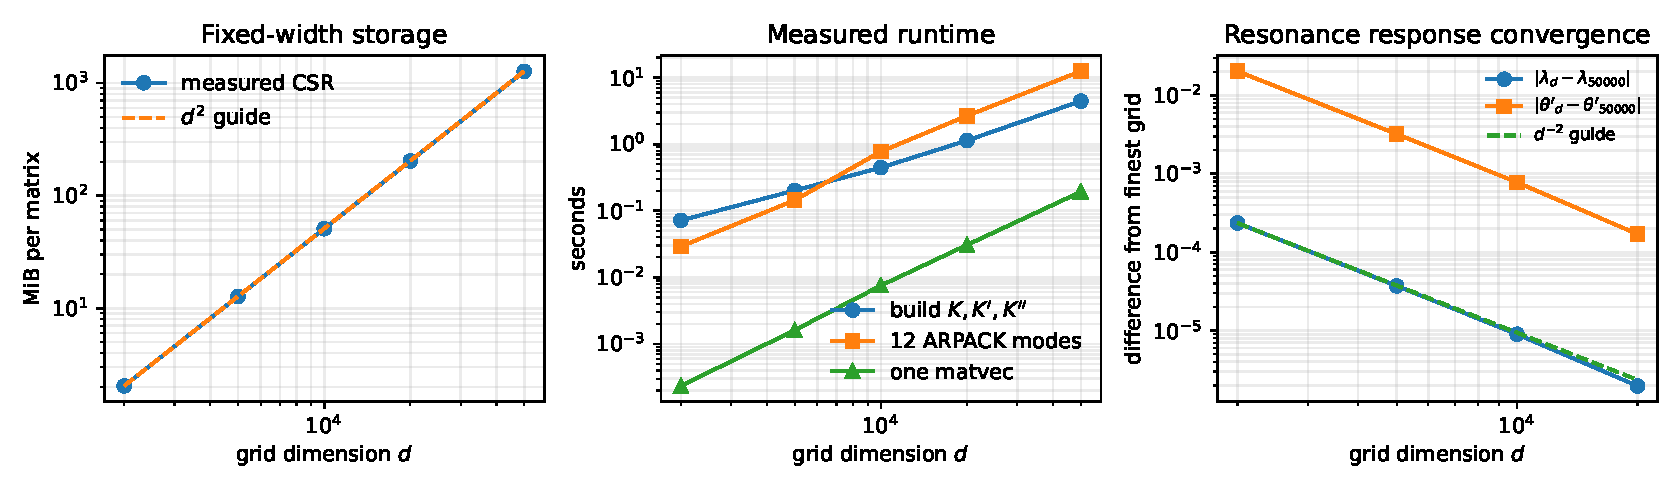
\includegraphics[width=\textwidth]{figures/operator_scaling.pdf}
\caption{Fixed-width resolution study.  Left: CSR storage is a small
fraction of dense storage but remains quadratic.  Middle: measured build,
Arnoldi, and matrix-vector times.  Right: the selected upper-half-plane
resonance and its analytic phase derivative exhibit second-order grid
convergence relative to the $d=50000$ computation.}
\label{fig:operator-scaling}
\end{figure}

\subsection{Weighted schedule scaling}

For a direct scalar test of the two weighted lemmas, use
$a_{n,T}=(n/T)^a$ with $a=0,1,3$, horizons from $10^3$ through $10^7$, and
$p=2$.  In the unanchored panel of \cref{fig:schedule-scaling}, every
coefficient
\[
  \frac{L_T^p}{\kappa}
  \frac{\sum_na_{n,T}\delta_n}{\sum_na_{n,T}}
\]
approaches one, although the convergence is only logarithmic.  In the
anchored panel, the scale is $L_T^{p+1}/(p\kappa)$ and the three limits are
$1$, $1/2$, and $1/4$, exactly as in \cref{cor:power}.  The finite-horizon
curves also warn against treating $T=10^6$ as asymptotic: the unweighted
anchored coefficient is still $1.324$ rather than $1$.

\begin{figure}[t]
\centering
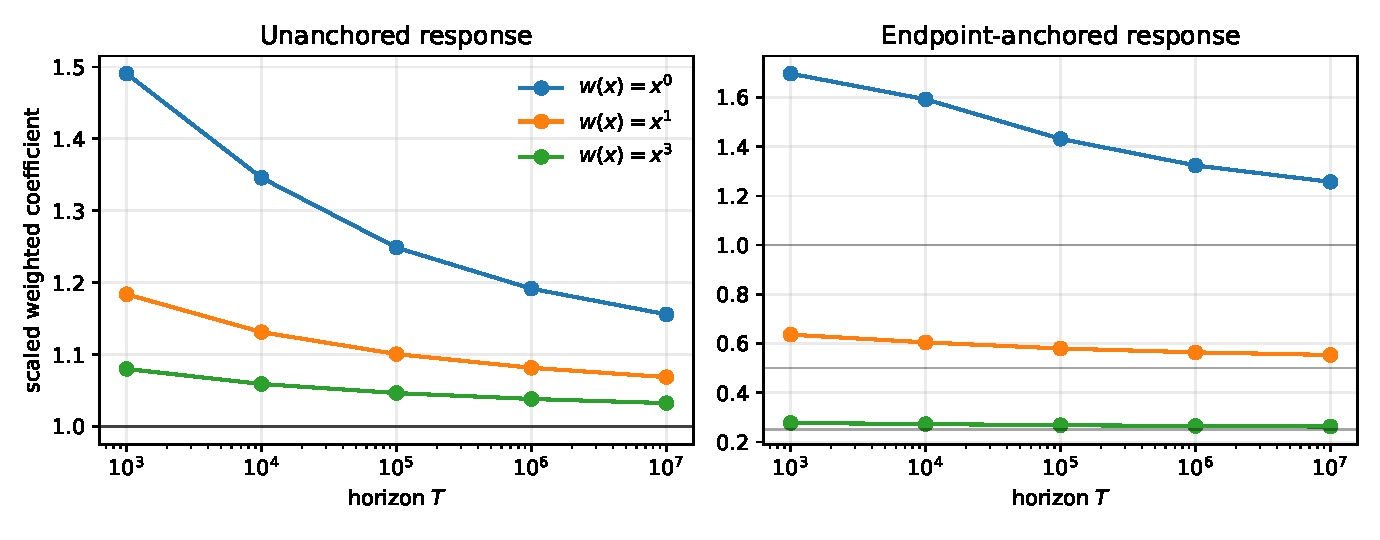
\includegraphics[width=0.88\textwidth]{figures/schedule_scaling.pdf}
\caption{Weighted logarithmic coefficients.  Unanchored driving forgets
every positive-density power weight at leading order.  Endpoint anchoring
removes that common term and exposes the logarithmic-age limits
$1/(a+1)$.  Horizontal lines show the theoretical limits.}
\label{fig:schedule-scaling}
\end{figure}

\section{Discussion}
\label{sec:discussion}

\subsection{What has been proved beyond operator freezing}

The previous fixed-resolution theorem applied to
$T^{-1}\sum_nK(u_n)$.  \Cref{thm:unanchored} now applies to the
row-normalized expected flow actually produced by propagating a probability
cloud.  Its assumptions are explicit: finite $d$, differentiability of the
matrix family, and positive time density for every retained source row.  For
a full Gaussian kernel on a compact parameter interval, positivity supplies
the density automatically; a hard sparse cutoff must be checked separately.
For a genuinely random finite-state Gaussian chain, \cref{cor:markov} shows
that the transition-count fluctuation is polynomially smaller than the
logarithmic response.  This is a rigorous positive extension, not merely a
numerical observation.

The extension also has a sharp boundary.  Endpoint anchoring cancels the
occupation-universal part.  The resulting diagonal age matrix $B$ enters
before spectral perturbation, so a single scalar calibration cannot in
general remove the bias.  Moreover, as the partition is refined, positive
occupation density and derivative bounds must be proved uniformly in the
chosen operator topology.  Neither follows from finite Gaussian positivity.

\subsection{What the computations do not establish}

The stable quantities in \cref{fig:operator-scaling} are finite-noise Markov
resonances.  Their convergence demonstrates that the discretized object is
numerically well posed at fixed $\sigma$.  It does not show that its phases
are self-adjoint energies, that an unbounded phase lift exists, or that its
resonances encode arithmetic fluctuations.  In particular:
\begin{itemize}[leftmargin=2em]
  \item no Riemann zero is loaded or compared in this study; however,
  $\sigma$ is inherited from a target-fitted exploratory scan and is
  explicitly not treated as target-independent;
  \item the eigenvalues lie inside the unit disk and belong to a nonnormal
  stochastic matrix;
  \item refining $d$ at fixed $\sigma$ approaches one noisy integral
  operator, whereas shrinking $\sigma$ approaches a different deterministic
  object; and
  \item a Hilbert--Polya claim would require an independently constructed
  self-adjoint operator and a complete spectral identity, neither of which is
  supplied here.
\end{itemize}

\subsection{Next theoretical step}

The present paper identifies and validates the first derivative retained by
long exposure.  Such an average forgets operator order.  A possible next
object is therefore a parity-resolved two-step cocycle or a centered trace
observable that survives after subtracting the frozen operator and the
occupation-age response.  Any arithmetic comparison should then be made
against independently unfolded zero fluctuations and under a controlled
joint limit in time, resolution, and noise width.  That bridge remains open.

\section{Conclusion}

Gaussian quadratic transfer matrices admit an exact and computationally
useful response calculus.  Their first and second derivatives are centered
score moments, hard cutoff has a twice-the-tail error, and simple resonance
response follows from left-right perturbation theory.  More importantly,
row-normalizing accumulated flow does not destroy the first response of an
unanchored logarithmic drive: positive-density source weights are too slowly
varying to alter its leading coefficient.  A finite-state Markov trajectory
inherits the result because its sampling error is polynomially smaller.

Endpoint anchoring changes the conclusion.  Once the universal slowly
varying component is canceled, rowwise logarithmic age appears at leading
order and modifies both eigenvalue and eigenphase response.  Resolution
scaling introduces a second distinction: fixed noise gives a well-defined
second-order continuum discretization with quadratic storage, while
cell-scaled noise gives linear storage by changing the limit and its
operator topology.

The 50,000-dimensional experiments validate these finite-matrix statements
without loading or comparing arithmetic target data, while retaining the
declared historically target-informed width.  They provide a rigorous and
reproducible foundation for studying renormalized dynamical resonances, while
placing no Riemann zeros in the spectrum and making no claim about the
Riemann hypothesis.

\section*{Data and code availability}

The manuscript source, tests, sparse implementation, machine-readable
benchmark outputs, and figure scripts are available at
\url{https://github.com/maris205/prime_dynamics_theory/tree/main/papers/renormalized-gaussian-response}.
The exact commands are listed in the accompanying README.

\section*{Acknowledgments}

The author acknowledges the use of an AI language model for assistance with
mathematical cross-checking, code auditing, manuscript organization, and
typesetting.  The author verified the final arguments and assumes
responsibility for the content.

{\small
\bibliographystyle{plainnat}
\bibliography{references}
}

\end{document}
